\documentclass{../khlslides}


\title[Fundamenten]{Conditionals}
\author{Fr\'ed\'eric Vogels}


\pgfkeys{/tikz/flowchart/node/.style={rectangle,fill=blue,opacity=0.5,text opacity=1,drop shadow,inner sep=2mm}}
\pgfkeys{/tikz/flowchart/arrow/.style={-latex,flowchart/arrowline}}
\pgfkeys{/tikz/flowchart/arrowline/.style={thick}}


\newcommand{\lcurly}{{\tt{\char '173}}}
\newcommand{\link}[2]{\href{#1}{\beamergotobutton{#2}}}
\newcommand{\PLACEHOLDER}[1]{\ensuremath{\langle}\textrm{\textit{#1}\ensuremath{\rangle}}}



\begin{document}

\begin{frame}
  \titlepage
\end{frame}

\begin{frame}
  \frametitle{Basiselementen Algoritmes}
  \begin{center}
    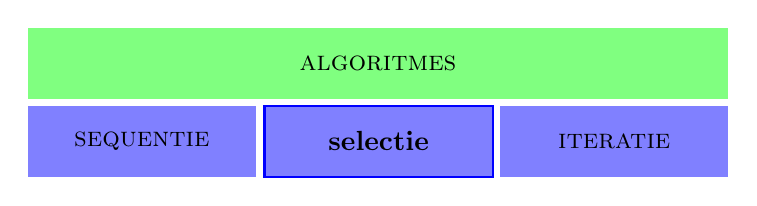
\begin{tikzpicture}[building block/.style={minimum width=2.9cm,minimum height=.9cm,fill=blue!50,font=\sc},
                        algorithm/.style={minimum width=8.9cm,minimum height=.9cm,fill=green!50,font=\sc}]
      \node[building block,anchor=south west] at (0,0) { sequentie };
      \node[building block,anchor=south west,draw=blue,thick] at (3,0) { \bfseries selectie };
      \node[building block,anchor=south west] at (6,0) { iteratie };
      \node[algorithm,anchor=south west] at (0,1) { algoritmes };
    \end{tikzpicture}
  \end{center}
\end{frame}

\begin{frame}
  \frametitle{Rad van Fortuin}
  \begin{center}
    \begin{tikzpicture}[scale=.9,transform shape]
      \path[use as bounding box] (-3,-3.5) rectangle (4,3);

      \foreach[count=\i] \text/\c in {50/red,100/blue,{\color{white}\sc\small bankroet}/black,500/yellow,125/green,250/purple,{\color{white}\sc\small bankroet}/black,1000/magenta,50/red,75/blue,250/brown,{\sc joker}/white,250/purple,25/cyan,{\sc verlies}/gray,100/blue,250/green,500/yellow} {
        \pgfmathparse{20}\let\deltaangle\pgfmathresult
        \pgfmathparse{\i * \deltaangle}\let\startangle\pgfmathresult
        \pgfmathparse{\startangle + \deltaangle/2}\let\midangle\pgfmathresult
        \pgfmathparse{\startangle + \deltaangle}\let\endangle\pgfmathresult
        \draw[fill=\c] (0,0) -- (\startangle:3cm) -- (\endangle:3cm) -- cycle;
        \coordinate (cell \i) at (\midangle:3cm);
        \node[anchor=east,rotate=\midangle] at (\midangle:3cm) {\text};
      }

      \draw[fill=black] (0,0) circle (.5cm);

      \node[anchor=south west] (note bankrupt) at ($ (cell 3) + (0.5,0.25) $) { \small {\tt score = 0; huidigeSpeler++;} };
      \draw[->] (cell 3) |- (note bankrupt);

      \node[anchor=south east] (note bankrupt 2) at ($ (cell 7) + (-0.5,0.25) $) { \parbox{3cm}{\raggedleft \small {\tt score = 0; \\ huidigeSpeler++;} } };
      \draw[->] (cell 7) |- (note bankrupt 2);

      \node[anchor=north east] (note joker) at ($ (cell 12) + (-0.5,-0.25) $) { \small {\tt jokers++;} };
      \draw[->] (cell 12) |- (note joker);

      \node[anchor=north west] (note pass) at ($ (cell 15) + (0.5,-0.25) $) { \small {\tt huidigeSpeler++;} };
      \draw[->] (cell 15) |- (note pass);

      \node[anchor=south west] (note 50) at ($ (cell 1) + (0.5,0.25) $) { \small {\tt score\ +=\ waarde;} };
      \draw[->] (cell 1) |- (note 50);
    \end{tikzpicture}
    \vskip2mm
    Uit te voeren berekening verschilt naargelang op welk segment men terecht komt
  \end{center}
\end{frame}

\begin{frame}
  \frametitle{Uitvoering Programma}
  \begin{center}
    \begin{tikzpicture}[scale=1.5,transform shape,
                        sequence point/.style={thick,blue!50,fill=white},
                        arc/.style={thick,blue!50},
                        execution/.style={ultra thick,black}]
      \path[use as bounding box] (0,-2) rectangle (7,2);

      \draw[arc] (0,0) -- (2,0);
      \foreach \y/\c/\p in {-1.5/{score = 0; huidigeSpeler++;}/below, -0.5/{jokers++;}/below, 1.5/{huidigeSpeler++;}/above, 0.5/{score += waarde;}/above} {
        \draw[arc] (2,0) -- (3,\y) -- (4,\y) node[midway,\p,black] {\tiny\tt \c} -- (5,0);
      }
      \draw[arc] (5,0) -- (7,0);

      \only<2->{
        \draw[execution] (0,0) -- (1,0);
      }
      \only<3->{
        \draw[execution] (1,0) -- (2,0);
      }
      \only<4->{
        \draw[execution] (2,0) -- (3,-.5);
      }
      \only<5->{
        \draw[execution] (3,-.5) -- (4,-.5);
      }
      \only<6->{
        \draw[execution] (4,-.5) -- (5,0);
      }
      \only<7->{
        \draw[execution] (5,0) -- (6,0);
      }
      \only<8->{
        \draw[execution] (6,0) -- (7,0);
      }

      \draw[sequence point] (0,0) circle (.05cm);
      \draw[sequence point] (1,0) circle (.05cm);
      \draw[sequence point] (2,0) circle (.05cm);
      \foreach \y in {-1.5,-0.5,0.5,1.5} {
        \draw[sequence point] (3,\y) circle (.05cm);
        \draw[sequence point] (4,\y) circle (.05cm);
      }
      \draw[sequence point] (5,0) circle (.05cm);
      \draw[sequence point] (6,0) circle (.05cm);
      \draw[sequence point] (7,0) circle (.05cm);

      \only<3>{
        \node[anchor=north east] (note) at ($ (2,0) + (-.5,-.5) $) {\parbox{2cm}{\raggedleft\tiny Stel dat speler op {\sc joker} beland is}};
        \draw (note.north east) -- (2,0);
      }
   \end{tikzpicture}
   \vskip5mm
   Slechts \'e\'en van de vier berekeningen moet uitgevoerd worden
  \end{center}
\end{frame}

\begin{frame}
  \frametitle{In Code}
  \begin{overprint}
    \onslide<1>
    \code[show lines,font size=\small,width=.9\linewidth]{if1.js}
    
    \onslide<2->
    \code[show lines,font size=\small,width=.9\linewidth]{if2.js}
  \end{overprint}

  \begin{tikzpicture}[overlay,remember picture]
    \only<3>{
      \draw[fill=red,opacity=.2] ($ (bankruptcy.south west) + (-.1,-.1) $) rectangle ($ (bankruptcy.north east) + (.1,.1) $);
      \draw[fill=red,opacity=.2] ($ (joker.south west) + (-.1,-.1) $) rectangle ($ (joker.north east) + (.1,.1) $);
      \draw[fill=red,opacity=.2] ($ (pass.south west) + (-.1,-.1) $) rectangle ($ (pass.north east) + (.1,.1) $);

      \node (note) at ($ (bankruptcy.north east) + (3,1) $) {Condities};
      \draw (note) -| (bankruptcy.north);
      \draw ($ (note.south west) ! 0.5 ! (note.south) $) -- ++(0,-1) -- (joker.east);
      \draw (note) -- ++(0,-2) -- (pass.east);

      \node (note 2) at ($ (else) + (3,-2) $) {\parbox{4cm}{\raggedright Indien aan geen van de condities voldaan wordt}};
      \draw (note 2) |- (else);
    }
  \end{tikzpicture}
\end{frame}

\begin{frame}
  \frametitle{Syntax en Semantiek}
  \begin{center}
    \begin{tikzpicture}
      \node[flowchart/node] (if) at (0,3) {evalueren \PLACEHOLDER{conditie}};
      \node[flowchart/node] (then) at (-2, 0) {uitvoeren \PLACEHOLDER{A}};
      \node[flowchart/node] (else) at (2, 0) {uitvoeren \PLACEHOLDER{B}};

      \draw[flowchart/arrow] ($ (if.north) + (0,1) $) -- (if.north);
      \draw[flowchart/arrow] (if.south) -- (0,2) -- ($ (then.north) + (0,0.5) $) node [midway,above,sloped] {true} -- (then.north);
      \draw[flowchart/arrow] (0,2) -- ($ (else.north) + (0,0.5) $) node [midway,above,sloped] {false} -- (else.north);

      \draw[flowchart/arrow] (then.south) -- ($ (then.south) - (0,0.5) $) -- (0,-2) -- (0,-3);
      \draw[flowchart/arrowline] (else.south) -- ($ (else.south) - (0,0.5) $) -- (0,-2);

      \node[anchor=west] at (3.5,1) {\parbox{4cm}{\code[font size=\small,width=.9\linewidth]{if.js}}};
    \end{tikzpicture}
  \end{center}
\end{frame}

\begin{frame}
  \frametitle{Syntax en Semantiek}
  \begin{center}
    \begin{tikzpicture}
      \node[flowchart/node] (if) at (0,3) {evalueren \PLACEHOLDER{conditie}};
      \node[flowchart/node] (then) at (-2, 0) {uitvoeren \PLACEHOLDER{A}};

      \draw[flowchart/arrow] ($ (if.north) + (0,1) $) -- (if.north);
      \draw[flowchart/arrow] (if.south) -- (0,2) -- ($ (then.north) + (0,0.5) $) node [midway,above,sloped] {true} -- (then.north);
      \draw[flowchart/arrow] (then.south) -- ($ (then.south) - (0,0.5) $) -- (0,-2) -- (0,-3);
      \draw[flowchart/arrowline] (0,2) -- (0,-2) node[midway,sloped,above] {false};

      \node[anchor=west] at (3.5,1) {\parbox{4cm}{\code[font size=\small,width=.9\linewidth]{if-no-else.js}}};
    \end{tikzpicture}
  \end{center}
\end{frame}

\begin{frame}
  \frametitle{Oefening}
  Waaraan is {\tt x} gelijk na uitvoering?
  \vskip4mm
  \code{exercise.js}
  \visible<2>{Na uitvoering is {\tt x = 10}.}
  \begin{tikzpicture}[overlay,remember picture]
    \only<2>{
      \draw[->] (assign 3.east) to[bend left=30] ($ (condition.east) + (.1,0) $)
                                to[bend left=30] (double.east)
                                to[bend left=45] (add 4.east);
    }
  \end{tikzpicture}
\end{frame}

\begin{frame}
  \frametitle{Oefening}
  Waaraan is {\tt y} gelijk na uitvoering?
  \vskip4mm
  \code{exercise2.js}
  \visible<2>{Na uitvoering is {\tt y = 2}.}
  \begin{tikzpicture}[overlay,remember picture]
    \only<2>{
      \draw[->] (assign x 3.east) to[bend left=60] ($ (declare y.east) + (.2,0) $)
                                  to[bend left=30] ($ (condition 1.east) + (.2,0) $)
                                  to[bend left=60] ($ (condition 2.east) + (.2,0) $)
                                  to[bend left=60] (assign y 2.east)
                                  to[bend left=45] (exit);
    }
  \end{tikzpicture}
\end{frame}

\begin{frame}
  \frametitle{Oefening}
  \code{ex-abs.js}
\end{frame}

\begin{frame}
  \frametitle{Inputs--Outputs}
  We stellen een input-output tabel op:
  \vskip4mm
  \begin{columns}
    \column{.6\linewidth}
    \begin{center}
      \begin{tabular}{c@{\hspace{1cm}}c}
        {\tt x} & {\tt abs} \\
        \toprule
        4 & \NODE{4}{r1} \\
        7 & \NODE{7}{r2} \\
        -4 &\NODE{4}{r3} \\
        3.7 & \NODE{3.7}{r4} \\
        -1.2 & \NODE{1.2}{r5} \\
        -5 & \NODE{5}{r6}
      \end{tabular}
    \end{center}
    \column{.4\linewidth}
  \end{columns}
  \vskip8mm

  \begin{overprint}
    \onslide<8>
    \begin{center}
        We identificeren twee verschillende berekeningen: \\
        {\tt abs = x} \hspace{.5cm} en \hspace{.5cm} {\tt abs = -x}
    \end{center}

    \onslide<9>
    \begin{center}
        Welke berekening moet uitgevoerd worden hangt af van {\tt x} \\
    \end{center}
  \end{overprint}
  
  \begin{tikzpicture}[remember picture,overlay]
    \foreach[count=\i] \sign in {,,-,,-,-} {
      \pgfmathparse{int(\i+1)}\let\slideindex\pgfmathresult
      \only<\slideindex->{
        \node[anchor=west] (note \i) at ($ (r\i) + (1,0) $) {\tt abs = \sign x};
        \draw[-latex] (note \i.west) -- +(-0.5,0);
      }
    }

    \only<9->{
      \node (pos) at ($ (note 2.east) + (2,0) $)  {\tt x > 0};
      \node (neg) at ($ (pos.south) + (0,-1) $)  {\tt x < 0};

      \foreach \to in {1,2,4} {
        \draw[-latex] (pos.west) -- (note \to.east);
      }
      \foreach \to in {3,5,6} {
        \draw[-latex] (neg.west) -- (note \to.east);
      }
    }
  \end{tikzpicture}
\end{frame}

\begin{frame}
  \frametitle{Absolute Waarde in JavaScript}
  \begin{overprint}
    \onslide<1-2>
    \code[width=.4\linewidth]{abs.js}

    \onslide<3-4>
    \code[width=.5\linewidth]{abs2.js}

    \onslide<5-6>
    \code[width=.5\linewidth]{abs3.js}

    \onslide<7-8>
    \code[width=.5\linewidth]{abs4.js}

    \onslide<9-10>
    \code[width=.5\linewidth]{abs5.js}

    \onslide<11>
    \code[width=.5\linewidth]{abs6.js}
  \end{overprint}

  \begin{overprint}
    \onslide<2>
    \begin{center}
      Wat indien {\tt x === 0}?
    \end{center}

    \onslide<4>
    \begin{center}
      Laatste test {\tt x === 0} is overbodig.
    \end{center}

    \onslide<6>
    \begin{center}
      Derde berekening is zelfde als eerste\dots
    \end{center}

    \onslide<8>
    \begin{center}
      Tweede test is nu nutteloos geworden
    \end{center}

    \onslide<10>
    \begin{center}
      Eerste test kan properder
    \end{center}
  \end{overprint}
\end{frame}

\begin{frame}
  \frametitle{Randgevallen}
  \begin{center} \scriptsize
    \begin{tabular}{lp{8cm}}
      \bf Martin:   & How about this, guys?  Bart can have it Mondays and Thursdays, Milhouse will get it Tuesdays and Fridays, and yours truly will take it Wednesdays and Saturdays. \\
      \bf Bart:     & Perfect! \\
      \bf Milhouse: & Wait a minute!  What about Sundays? \\
      \bf Bart:     & [suspiciously] Yeah, what \emph{about} Sundays? \\
      \bf Martin:   & Well, Sunday possession will be determined by a random number
                generator.  I will take the digits 1 through 3, Milhouse will
                have 4 through 6, and Bart will have 7 through 9. \\
      \bf Bart:     & Perfect! \\
      \bf Milhouse: & Wait a minute!  What about 0? \\
      \bf Bart:     & [suspiciously] Yeah, what \emph{about} 0? \\
      \bf Milhouse: & Yeah. \\
      \bf Martin:   & Well, in the unlikely event of a 0, possession will be determined
                  by Rock Scissors Paper competition, best 3 out of 5.  How's that? \\
      \bf Bart and & Oh, okay. \\
      \bf Milhouse: & Yeah, all right.
    \end{tabular}
  \end{center}
  \begin{center}
    
\includegraphics[width=3cm]{simpsons.png}
  \end{center}
\end{frame}



\end{document}

%%% Local Variables: 
%%% mode: latex
%%% TeX-master: t
%%% End: 
